\documentclass[10 pt,usenames,dvipsnames, oneside]{article}
\usepackage{../../../modelo-ensino-medio}


\begin{document}

\begin{center}
  \begin{minipage}[l]{3cm}
\includegraphics[width=2cm]{logo}    
\end{minipage}\hfill
\begin{minipage}[r]{.8\textwidth}
 {\Large \scshape Atividade: Hora de encher a piscina}  
\end{minipage}
\end{center}
\vspace{.2cm}

\ifdefined\prof
\begin{objetivos}
\item \textbf{LAF3} Calcular e interpretar a taxa de variação média de uma função em um intervalo dado, tanto algebricamente quanto a partir de dados gráficos ou de uma tabela, identificando tendências de crescimento e decrescimento.
\end{objetivos}

\begin{goals}
\begin{enumerate}

\item [OE1] Utilizar o vocabulário associado ao conceito de taxa de variação para descrever com palavras uma situação real (item a).

\item [OE2] Associar uma situação real a uma representação gráfica (item b).

\item [OE3] Diferenciar situações de crescimento, identificando quando o gráfico pode ser uma linha reta – taxa de variação constante (item a) e quando não (item b).

\end{enumerate}

\tcblower
\begin{itemize}
\item É importante que o estudante perceba que no item a), tanto na primeira parte do
enchimento quanto na segunda parte, a profundidade $d$ aumenta uniformemente. É
desejável que eles se expressem utilizando expressões como “$d$ aumenta
uniformemente”.
\item Ainda no item a), é esperado que o estudante perceba que há uma mudança na taxa em
que $d$ aumenta. Isto é, na primeira parte do enchimento da piscina a profundidade $d$
aumenta mais rapidamente do que na segunda parte do enchimento.
\item Para o item b) há algumas possibilidades de gráficos que representam corretamente a
situação. É importante observar se os estudantes perceberam que o gráfico começa em
$(0,0)$, termina em $(30,2)$ e apresenta uma mudança em $(x, 1)$, com $5\leq x \leq 10$, por
exemplo.
\item Após a realização da atividade discuta com os estudantes sobre a justificativa para o
gráfico que representa a primeira parte do enchimento no item b) ser curvo com
concavidade voltada para baixo.
\end{itemize}

\end{goals}

\bigskip
\begin{center}
{\large \scshape Atividade}
\end{center}
\fi

Uma piscina retangular está sendo cheia com uma mangueira que fornece água a uma taxa constante. Uma seção transversal da piscina é mostrada na imagem a seguir.

\begin{figure}[H]
\centering
\includegraphics[width=300bp]{taxa-ativ-3-1}
\end{figure}

\begin{enumerate}
\item Descreva em palavras como a profundidade $d$, da água até o fundo da piscina, varia com o tempo, a partir do momento em que a piscina vazia começa a encher.
\item Uma piscina retangular está sendo cheia de maneira semelhante.

\begin{figure}[H]
\centering
\includegraphics[width=300bp]{taxa-ativ-3-2}

\end{figure}

Supondo que a piscina leva 30 minutos para encher até a borda. Esboce um gráfico para mostrar como a profundidade $d$, da água até o fundo da piscina, varia com o tempo, a partir do momento em que a piscina está vazia.

\begin{figure}[H]
\centering

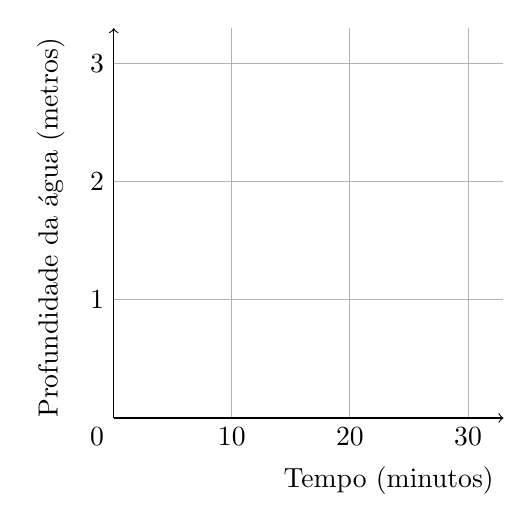
\begin{tikzpicture}[scale=1.5]
\draw [gray!60] (0,0) grid (3.3,3.3);
\draw [->] (0,0) -- (3.3,0) node [below left, shift={(0,-.5)}] {Tempo (minutos)};
\draw [->] (0,0) -- (0,3.3) node [above left, shift={(-.5,0)}, rotate=90] {Profundidade da água (metros)};
\foreach \x in {1,2,3}{
  \node [below] at (\x,0) {\x0};
  \node [left] at (0,\x) {\x};
};
\node [below left] at (0,0) {0};
\end{tikzpicture}
\end{figure}
\end{enumerate}

\ifdefined\prof

\begin{solucao}
\begin{enumerate}
\item A profundidade de $d$, da água até o fundo da piscina, aumenta uniformemente na primeira parte do enchimento. Após o enchimento dessa parte mais estreita há uma mudança na taxa com que $d$ aumenta, nesse segundo momento $d$ aumentará mais lentamente, porém esse aumento também ocorrerá de forma uniforme.

\item Um gráfico possível é:

\begin{tikzpicture}[scale=1.5, every node/.style={black},every path/.style={black}]
\draw [gray!60] (0,0) grid (3.3,3.3);
\draw [->] (0,0) -- (3.3,0) node [below left, shift={(0,-.5)}] {Tempo (minutos)};
\draw [->] (0,0) -- (0,3.3) node [above left, shift={(-.5,0)}, rotate=90] {Profundidade da água (metros)};
\foreach \x in {1,2,3}{
  \node [below] at (\x,0) {\x0};
  \node [left] at (0,\x) {\x};
};
\node [below left] at (0,0) {0};
\draw [session1, thick] (1,1) -- (3,2);
\fill (3,2) circle (1pt);
\draw [session3, domain=0:1, thick] plot (\x,{-(\x)^2+2*\x});
\end{tikzpicture}
\end{enumerate}


\end{solucao}
\fi

\end{document}